\documentclass[a4paper, 12pt]{article}
\usepackage{graphicx}
\usepackage{listings}
\usepackage{tikz}
\usetikzlibrary{automata, positioning, arrows}


\setlength\parindent{24pt}

\lstset{language=python,breaklines=true, frame=single}
\tikzset{
        ->,  % makes the edges directed
        %>=stealth’, % makes the arrow heads bold
        node distance=5cm, % specifies the minimum distance between two nodes. Change if n
        every state/.style={thick, fill=gray!10}, % sets the properties for each ’state’ n
        initial text=$ $, % sets the text that appears on the start arrow
        }

\begin{document}
\begin{figure}
    \centering
    \includegraphics[width=1\textwidth]{Logo}
\end{figure}

\title{CPS3233 Assignment Report}
\author{Manwel Bugeja}
\date{\today}
\maketitle
  
\tableofcontents
\newpage

\section{Elevator System Specification}
In this section, the specifications of the elevator system are expressed in several different formal notations. The notations are Finite State Automata (FSAs), Regular Expressions (RE), Timed Automata (TAs) and Duration Calculus (DC). From the ones listed, TAs and DC are the capable of expressing timed events. \\

\subsection{Finite State Automata}
A finite state automata was designed to describe the elevator system. The formal definition of the state machine can be seen in listing \ref{lst:FSA}. The lift can be in one of three states: Idle, Loading or Moving. Idle is when the lift is not moving and has its door closed. Loading when the lift is not moving but has the doors open. Moving is when the lift is moving either up or down. Note that a 'bad' state could be added for when the lift is moving and has the doors open as the lift should never be in this state. \\



\begin{lstlisting}[
caption={FSA definition}
\label{lst:FSA}
]
M = {
{Idle, Loading, Moving},
{openDoor, closeDoor, stop, goUp, goDown},
{
    Idle, openDoor -> Loading,
    Idle, goUp -> Moving,
    Idle, goDown -> Moving,
    Loading, closeDoor -> Idle,
    Moving, stop -> Idle
},
Idle,
{}
}
\end{lstlisting}





\begin{figure}[ht] % ’ht’ tells LaTeX to place the figure ’here’ or at the top of the page
    \centering % centers the figure
    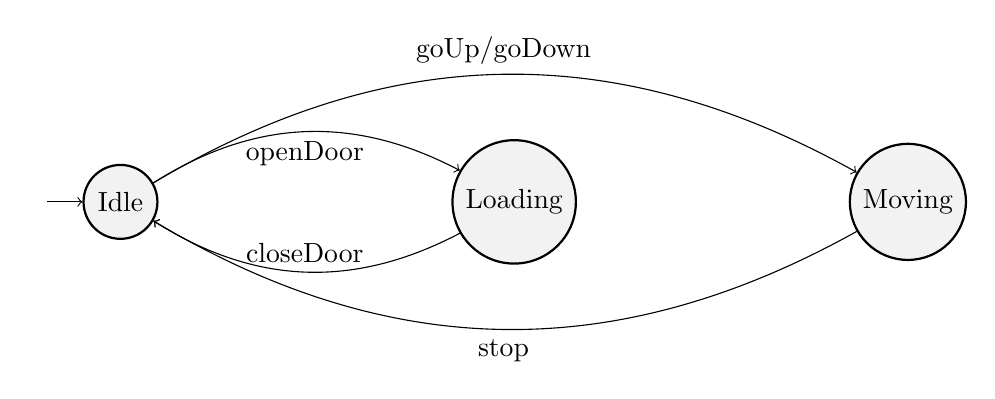
\begin{tikzpicture}
        % tikz code goes here
        \node[state, initial] (Idle) {Idle};
        \node[state, right of=Idle] (Loading) {Loading};
        \node[state, right of=Loading] (Moving) {Moving};
        
        \draw (Idle) edge[bend left, below] node{openDoor} (Loading);
        \draw (Loading) edge[bend left, above] node{closeDoor} (Idle);
       	\draw (Idle) edge[bend left, above] node{goUp/goDown} (Moving);
	\draw (Moving) edge[bend left, below] node{stop} (Idle);
        
    \end{tikzpicture}
    \caption{Caption of the FSM}
    \label{fig:my_label}
\end{figure}



\subsection{Regular Expressions}
\subsection{Timed Automata}
\subsection{Duration Calculus}


\section{Runtime Verification}

\section{Model-Based Testing}

\section{Runtime Verification and Testing}

\bibliographystyle{abbrv}
 \bibliography{references}

\end{document}
